\documentclass{beamer}
\usetheme{metropolis}

\usepackage{luatexja}
\usepackage[ipaex]{luatexja-preset}
\usepackage{listings}
\renewcommand{\kanjifamilydefault}{\gtdefault}

\title{\bfseries ISUCON本ゆる輪読会 \#1}
\subtitle{\bfseries Chapter2 モニタリング}
\author{aoshima}
\date{2022年8月14日}
\subject{モニタリング}

\begin{document}

\begin{frame}
  \titlepage
\end{frame}

\begin{frame}{今日の資料}
  \href{https://github.com/aoshimash/techresi-isucon-workshop}{https://github.com/aoshimash/techresi-isucon-workshop}
\end{frame}

\begin{frame}{モニタリングとは}
  \begin{quote}
    Webサービスを提供する側にとってのモニタリングは、Webアプリケーションやそれらを提供する基盤となる部分の状態を計測するという意味合いで使われます。
  \end{quote}
  モニタリングは高速化の対象がどのように遅くなっているのかを正しく把握するために重要な作業。
\end{frame}

\begin{frame}{モニタリングに対する考え方}
  重要なこと
  \begin{itemize}
    \item 変わらない視点でモニタリングすること
    \item モニタリングする目的を確実に定めて、チーム内で共有すること
    \item メトリクスをダッシュボード化しておくこと(過去のデータをみたり複数のメトリクスの動きを同時に確認するため)
  \end{itemize}
\end{frame}

\begin{frame}{モニタリングの種類}
  モニタリングは大きく2つに分けることができる。
  \begin{block}{外形監視}
    アプリケーションを外側からモニタリングする手法。サービスが正しく動作しているかを確かめることが主な目的。
  \end{block}
  \begin{block}{内部監視}
    アプリケーションの内側からモニタリングする手法。ユーザーが見えない部分の状態をモニタリングし、それらが意図しない状態になっていないかを確かめることが主な目的。
  \end{block}
\end{frame}

\begin{frame}{外形監視}
  提供しているHTTPエンドポイントに対して実際にHTTPリクエストを行う。(ISUCONのベンチマークもこれ)
  \begin{figure}
    \centering
    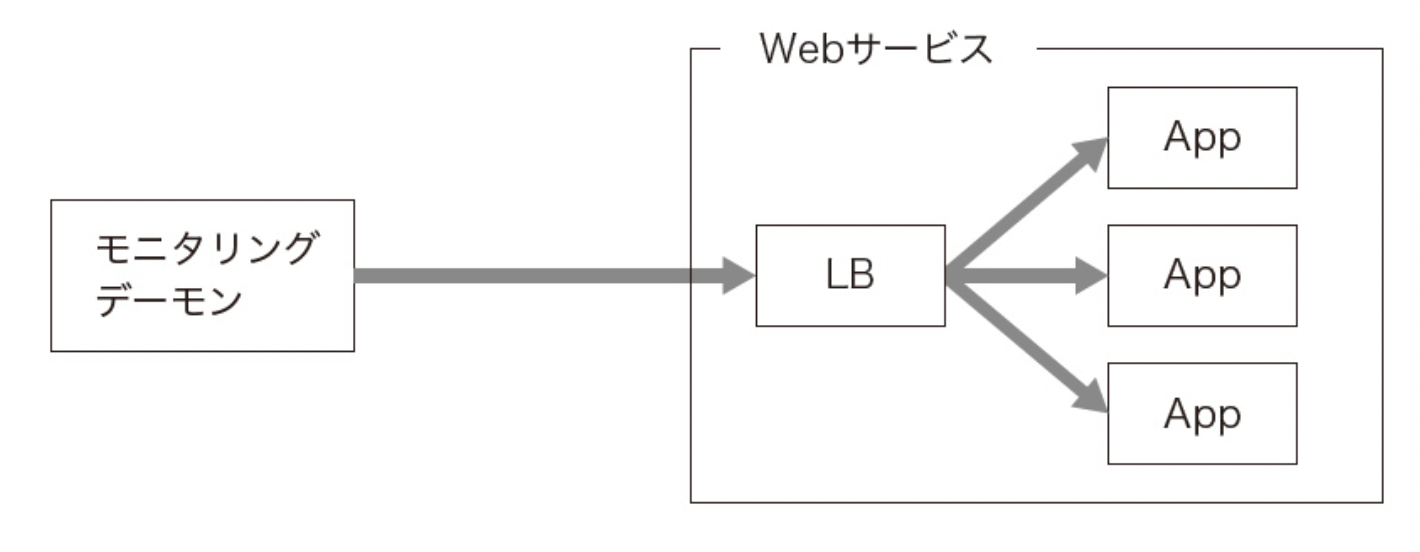
\includegraphics[clip, keepaspectratio, width=90mm]{./fig/external_monitoring.png}
  \end{figure}
\end{frame}

\begin{frame}{内部監視}
  WebアプリケーションやOS、ミドルウェアのメトリクスを確認する。
  \begin{figure}
    \centering
    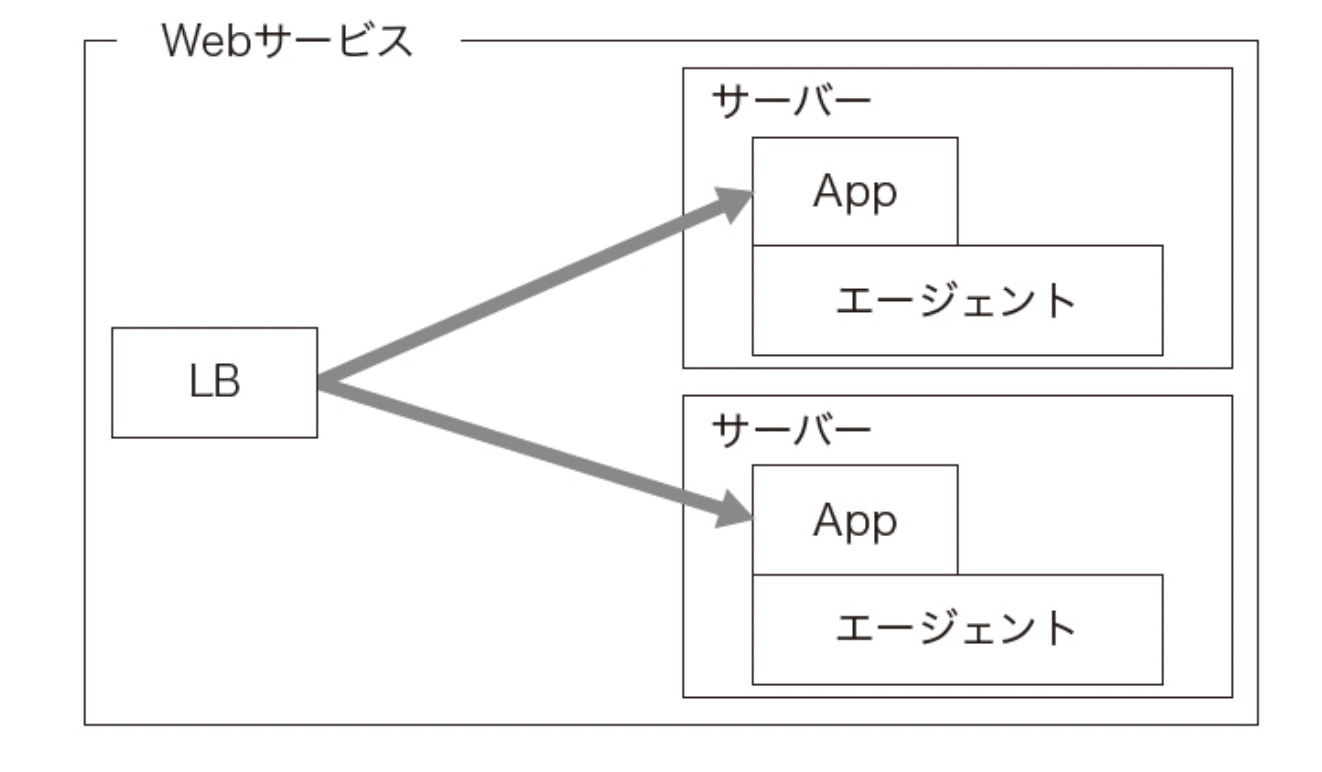
\includegraphics[clip, keepaspectratio, width=90mm]{./fig/internal_monitoring.png}
  \end{figure}
\end{frame}

\begin{frame}{手動での監視}
  Linuxコマンドで簡単な内部監視をしてみよう!
  \begin{itemize}
    \item top: CPU使用率
    \item free: メモリ使用率
  \end{itemize}
\end{frame}

\begin{frame}{top系コマンド}
  topとかfreeをそのまま使うより、こういうコマンド使うほうが便利。
  \begin{itemize}
    \item \href{https://htop.dev}{htop}
    \item \href{https://ctop.sh/}{ctop}
    \item \href{https://github.com/aksakalli/gtop}{gtop}
    \item \href{https://github.com/nicolargo/glances}{glances}
  \end{itemize}
  他にも色々あるらしい。
  「\href{https://qiita.com/bezeklik/items/980d987ad0afd264bfb0}{top系モニタリングツールまとめ}」
\end{frame}

\begin{frame}{topのヘッダ}
  \begin{itemize}
    \item PID: プロセスID
    \item USER: プロセスオーナー
    \item PRI: 優先順位
    \item NI: nice値
    \item VIRT: 仮想メモリのサイズ
    \item RES: プロセスが実際に使っているメモリサイズ
    \item SHR: プロセスの共有メモリのサイズ
    \item S: プロセスの状態 (S: スリープ, R: 実行中, D: ディスクスリープ, Z: ゾンビ, T: トレースまたは一時停止, W: ページング)
    \item CPU$\%$: 使用しているCPU時間のパーセンテージ
    \item MEM$\%$: 使用しているメモリのパーセンテージ
    \item TIME+: プロセスがユーザとシステムに費やした時間
  \end{itemize}
\end{frame}

\begin{frame}{モニタリングツール}
  本番環境では手動でのモニタリングだけではなく、モニタリングツールと呼ばれるソフトウェアまたはSaaSを使うことが多い。モニタリングツールは次のような機能をもつ。
  \begin{itemize}
    \item メトリクスを自動で収集し、保存する
    \item 保存したメトリクスをWebブラウザなどで時系列順に表示する・集計用のクエリなどで表示を切り替えられる
    \item メトリクスが特定の閾値に達すると通知を行う
  \end{itemize}
\end{frame}

\begin{frame}{モニタリングツールのアーキテクチャ}
  大きく分けて2つのアーキテクチャがある。
  \begin{itemize}
    \item プル型
    \item プッシュ型
  \end{itemize}
  どちらが優れているというわけではなく、特徴を理解して自分の環境に合ってるものを選べばいい。
\end{frame}

\begin{frame}{プル型}
  モニタリングアプリケーションからエージェントに対してメトリクス取得をリクエストするアーキテクチャ。
  \begin{figure}
    \centering
    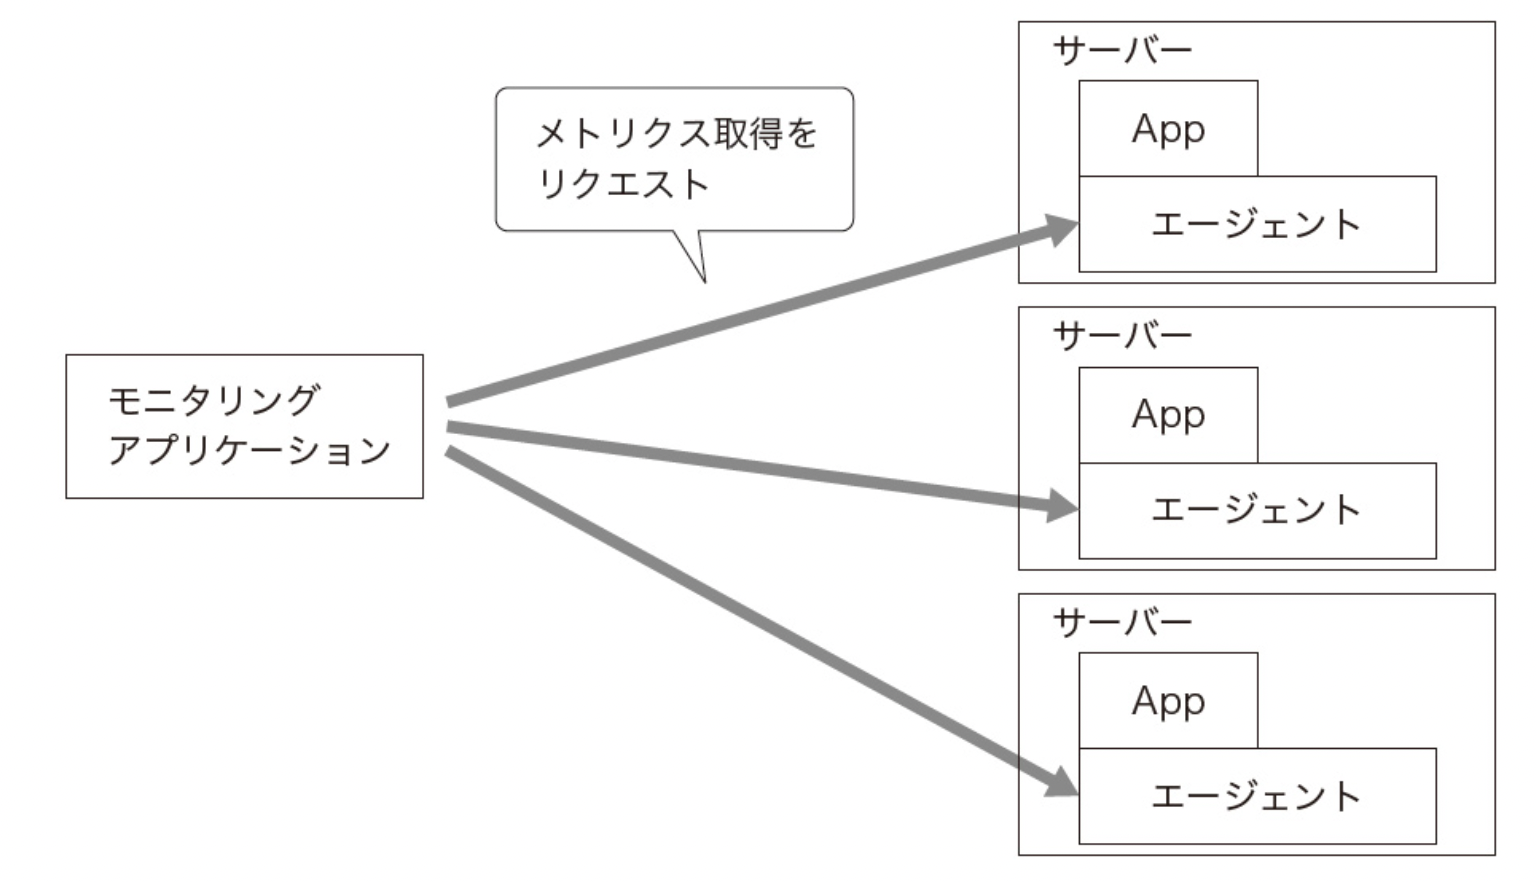
\includegraphics[clip, keepaspectratio, width=70mm]{./fig/pull.png}
  \end{figure}
  メリットはエージェント側の実装をシンプルにできること。(例: Prometheus, Nagios, Zabbix)
\end{frame}

\begin{frame}{プッシュ型}
  エージェントからモニタリングアプリケーションにメトリクスを送信するアーキテクチャ。
  \begin{figure}
    \centering
    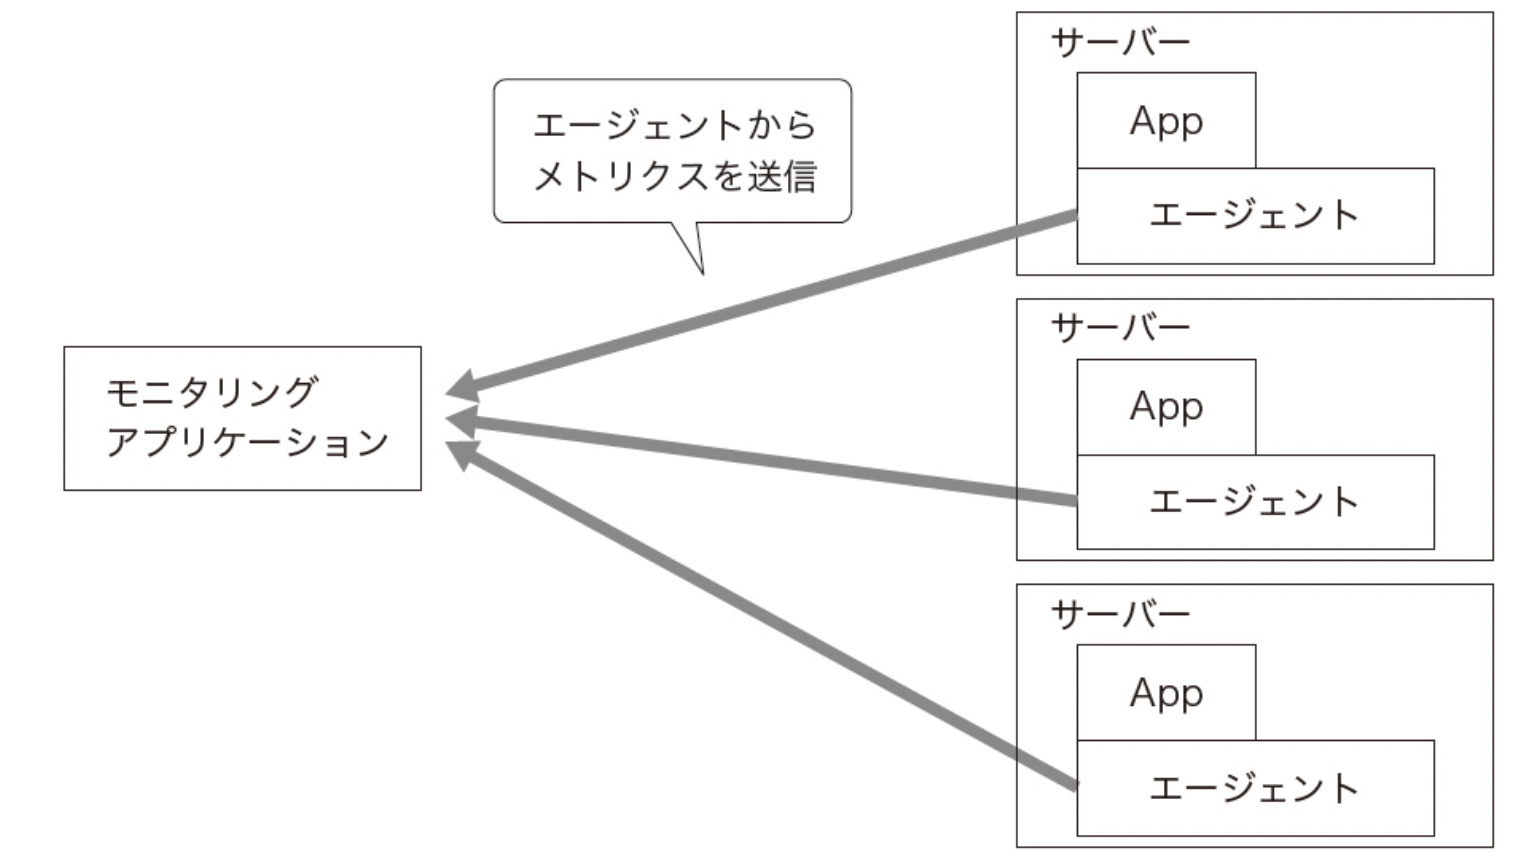
\includegraphics[clip, keepaspectratio, width=70mm]{./fig/push.png}
  \end{figure}
  メリットはモニタリングアプリケーション用のポート開放が要らないところと、モニタリング対象の増減時にモニタリングアプリケーション側の設定変更が要らないところ。(例: Datadog, Mackerl, Sensu)
\end{frame}

\begin{frame}{Prometheusをさわってみよう}
  モニタリングツールの一例としてPrometheusを実際にさわってみよう!\\
  Prometheusの特徴
  \begin{itemize}
    \item プル型(Pushgatewayを使ってプッシュ型として動かすこともできる)
    \item ServiceDiscoveryによってモニタリング対象の増減時に自動で対応できる
    \item セルフホストもできるしSaaSもある
  \end{itemize}
\end{frame}

\begin{frame}{node\_exporter}
  node\_exporeterhはPrometheusにおけるエージェントの一つ。Linuxにおけるシステムメトリクスを取得することができ、Linuxホスト1台につき1つずつインストールされる。
  モニタリングアプリケーションであるPrometheusからメトリクスを取得するためのリクエストを受け取ると、現在の状態を収集してHTTPレスポンスとして返却する。
\end{frame}

\begin{frame}[fragile]{検証環境の立ち上げ}
  検証環境用のdocker-composeをexampleディレクトリに用意したので、まずは次のコマンドで環境を立ち上げる。

  \begin{lstlisting}[language=bash]
    $ docker-compose up -d
  \end{lstlisting}

  これで、node\_exporterを含めていくつかのコンテナが立ち上がる。
  curlでnode\_exporterにGETしてみる。

  \begin{lstlisting}[language=bash]
    $ curl localhost:9100/metrics
  \end{lstlisting}

  ちなみに、このHTTPレスポンスのフォーマットはOpenMetricsという標準化されたフォーマット。
\end{frame}

\begin{frame}{node\_exporterで取得できるメトリクス}
  node\_exporterで取得できるメトリクスはここで確認できる。\\
  \href{https://github.com/prometheus/node\_exporter}{https://github.com/prometheus/node\_exporter}\\
  Prometehusに保存するメトリクスが増えるほど、サーバーの負荷が増え、ディスク容量も圧迫するため、どのメトリクスを取得するのか取捨選択は必要。
\end{frame}

\begin{frame}{Prometheusダッシュボード}
  \href{http://localhost:9090}{http://localhost:9090} \\
\end{frame}

\begin{frame}[fragile]{PromQL}
  PromQL(Prometheus Query Language)をテキストボックスに入力してグラフを出力する。\\
  CPU利用時間を表示するクエリ
  \begin{lstlisting}[basicstyle=\tiny]
    avg without(cpu) (rate(node_cpu_seconds_total{mode!="idle"}[1m]))
  \end{lstlisting}
\end{frame}

\begin{frame}{Grafanaの紹介}
  Grafanaを使うとPrometheusのデータを使ってダッシュボードを作ることができて便利!\\
  \href{http://localhost:3000}{http://localhost:3000} \\
  初期ユーザーのパスワードは admin/admin\\
  ダッシュボードのサンプルは、"Configuration > Data sources > Prometheus > Dashboards" から 「Promethus 2.0 Stats」をimportするとみることができる。
\end{frame}

\begin{frame}{モニタリングの注意点}
  プロファイラとかちゃんと使うと良さそう。Goだと\href{https://pkg.go.dev/net/http/pprof}{pprof}とかかな?
\end{frame}

\begin{frame}{ログに対するモニタリング}
  パフォーマンスチューニングの文脈では、
  \begin{itemize}
    \item アクセスログに記録されるリクエストごとのレイテンシ
    \item エラーログ
  \end{itemize}
  などがとくに大事
\end{frame}

\end{document}
